\section{Sharing Data Between Clusters with CharonFS}
\label{charonfs}
\textsc{Charon} is a cloud-backed file system capable of storing and sharing big data in a secure, reliable, and efficient way using multiple cloud providers and storage repositories. 
It is secure and reliable because it does not require trust on any single entity, and it supports the storage of different types of data in distinct locations to comply with required privacy premises. 
Two distinguishing features of \textsc{Charon} are its serverless design (no client-managed server is required in the cloud) and its efficient management of large files (by employing prefetching, cache, and background writes).

Figure~\ref{fig:charon} illustrates a deployment scenario where two biobanks store their data in local repositories, in single public cloud providers, and in a resilient cloud-of-clouds. 
In this scenario, the namespace tree has six nodes: directories \texttt{d1} and \texttt{d2}, and files \texttt{A}, \texttt{B}, \texttt{C}, and \texttt{D}. 
The namespace is maintained in the cloud-of-clouds, together with file \texttt{B}.
File \texttt{D}, less critical, is kept in a single cloud.
File \texttt{A} is stored locally because it cannot leave Biobank 2. 
File \texttt{C} is shared between the two sites (e.g., in the same country), thus being stored in both of them.

% \vspace{-5mm}
\begin{figure}[ht]
 \centering
 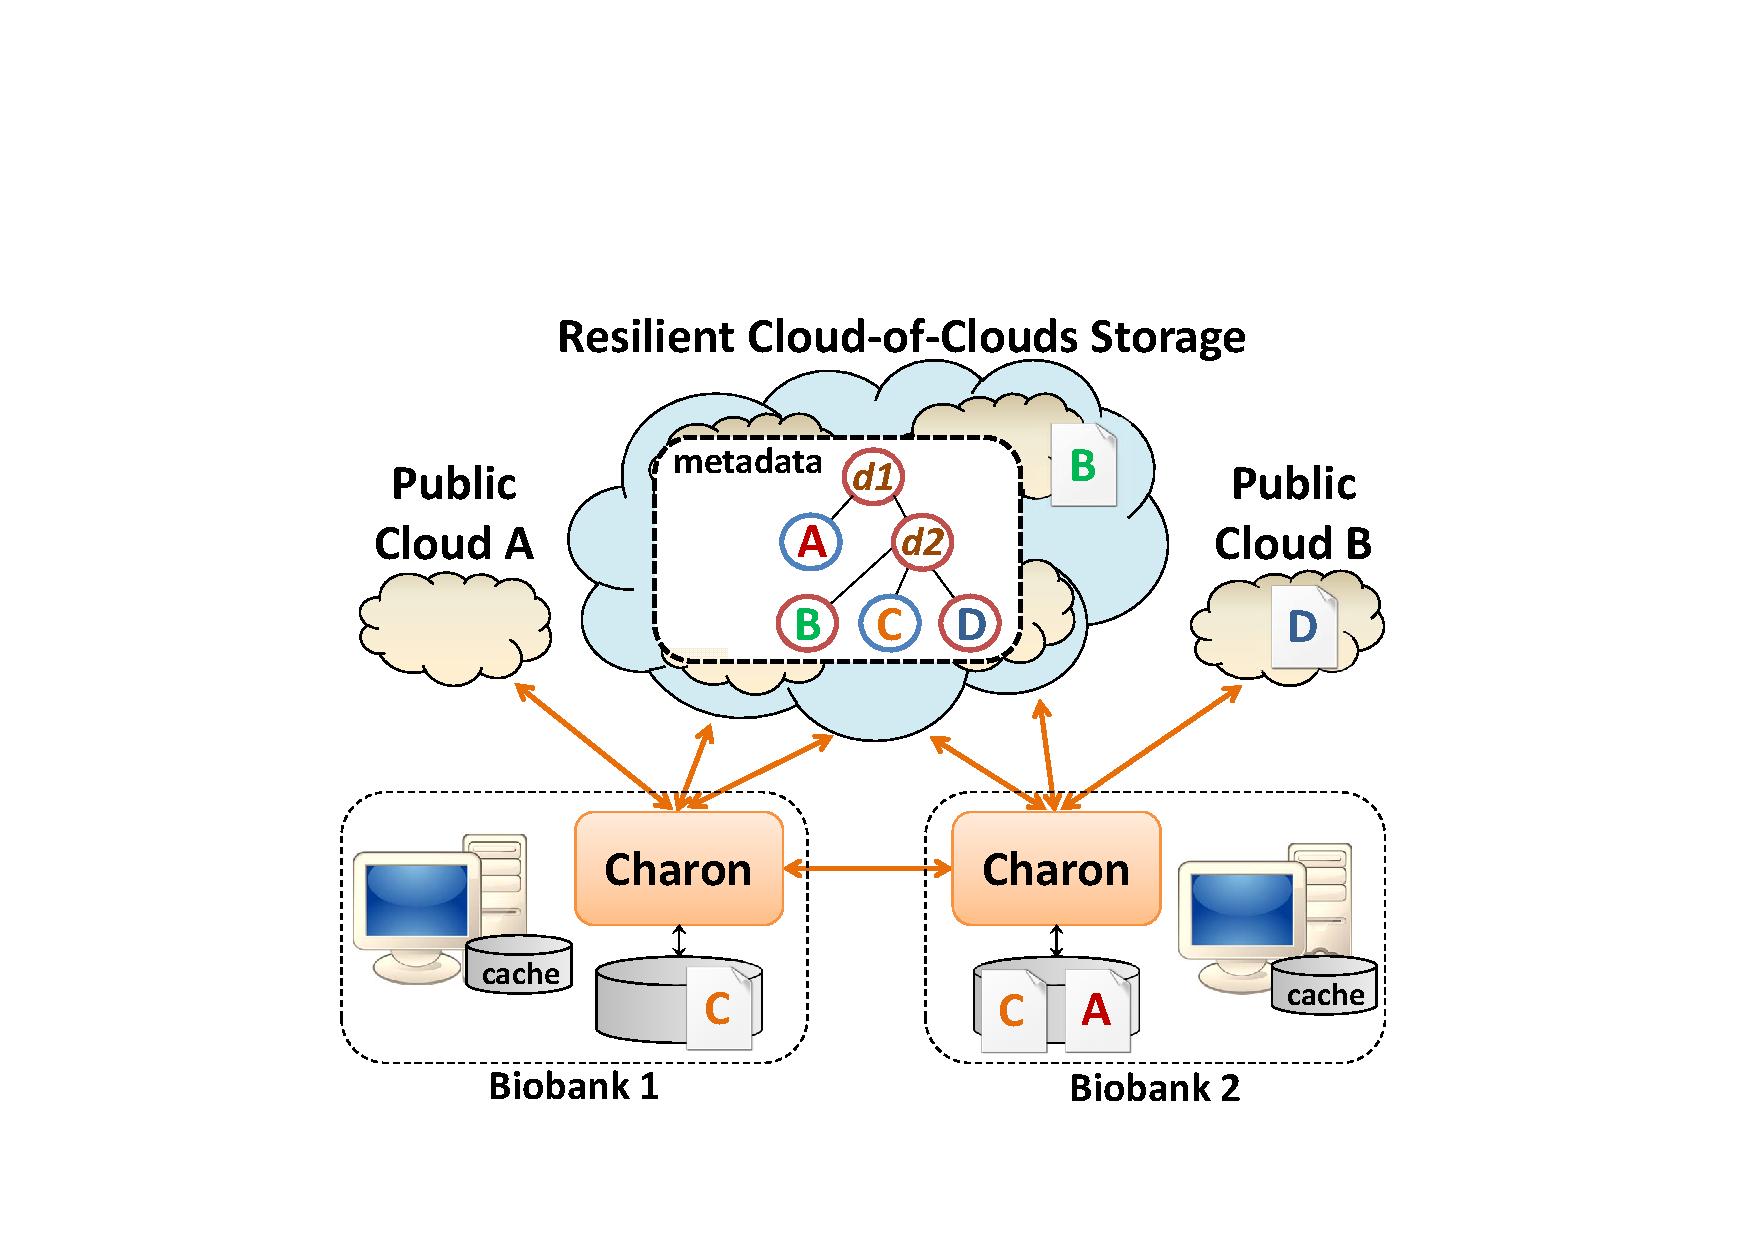
\includegraphics[width=0.5\columnwidth]{./imgs/charon_arch.pdf}
 % charon_arch.pdf: 0x0 pixel, 300dpi, 0.00x0.00 cm, bb=
\caption{\small \textsc{Charon} overview.}
\label{fig:charon}
\end{figure}
% \vspace{-5mm}

The BiobankCloud platform is able to process data stored in HopsFS, which has a view of all data being stored in a single cluster. \textsc{Charon} performs the inter-datacenter tasks and the processes between Biobanks and public clouds.
% In the next section, we discuss the integration between these two storage systems and evaluate the most appropriate integration scenario for the BiobankCloud platform.
